\documentclass{article}

\usepackage{fancyhdr} % Required for custom headers
\usepackage{lastpage} % Required to determine the last page for the footer
\usepackage{extramarks} % Required for headers and footers
\usepackage[usenames,dvipsnames]{color} % Required for custom colors
\usepackage{graphicx} % Required to insert images
\usepackage{listings} % Required for insertion of code
\usepackage{courier} % Required for the courier font
\usepackage{listings}
\usepackage{amsmath,xparse}
\usepackage{fontspec}
\usepackage[boldfont,slantfont]{xeCJK}
\usepackage[cs4size,UTF8,winfonts,heading=true]{ctex}
% \usepackage{xifthen, xparse, xstring, fancyhdr, etoolbox}
% \usepackage{indentfirst}
% \usepackage{mwe}
\usepackage{tikz}
\usepackage{forest}
% \usepackage{zh_CN-Adobefonts_internal}
\setlength{\parindent}{4em}
\addtolength{\parskip}{3pt}


% Margins
\topmargin=-0.45in
\evensidemargin=0in
\oddsidemargin=0in
\textwidth=6.5in
\textheight=9.0in
\headsep=0.25in
\headheight=13pt

\linespread{1.1} % Line spacing

% Set up the header and footer
\pagestyle{fancy}
\lhead{网络安全一班} % Top left header
\chead{\hmwkClass\ \hmwkTitle} % Top center head
\rhead{3019244283 谢远峰 } % Top right header
\lfoot{\lastxmark} % Bottom left footer
\cfoot{} % Bottom center footer
\rfoot{第\ \thepage\ 页} % Bottom right footer
\renewcommand\headrulewidth{0.4pt} % Size of the header rule
\renewcommand\footrulewidth{0.4pt} % Size of the footer rule
\renewcommand{\normalsize}{\fontsize{12.5pt}{\baselineskip}\selectfont}
\renewcommand{\contentsname}{目录} % Use 目录 instead of Content



%--Edit Title, Author and Date here

\newcommand{\hmwkTitle}{编译原理-文法基础} % Assignment title
% \newcommand{\hmwkSupplement}{无约束单目标优化问题} % Due date
\newcommand{\hmwkClass}{} % Course/class
\newcommand{\hmwkClassTime}{\today} % Class/lecture time
\newcommand{\hmwkAuthorName}{网安一班\ 3019244283\ 谢远峰 } % Your name

\title{
\vspace{2in}
\huge{\textbf{\hmwkClass \  \hmwkTitle}}\\
% \Large\vspace{0.1in}\large{\hmwkSupplement}\\
\vspace{2.5in}
}

\author{\textbf{\hmwkAuthorName}}
\date{\hmwkClassTime}

%----------------------------------------------------------------------------------------

\begin{document}

\maketitle
\thispagestyle{empty}
%---Following Are Contents---

% \newpage
% \tableofcontents
\newpage

\section{文法基础}
\subsection{}
\noindent
令文法 $G_1[N]:N \rightarrow D |ND \ ; \ D \rightarrow 0|1|2|3|4|5|6|7|8|9$\\
(1) $G_1[N]$的语言$L(G_1)$是什么? \\
(2) 改造该文法,使其产生正整数?\par
\noindent
(1)最左推导:
\begin{align*}
       & N \rightarrow ND \rightarrow NDD \rightarrow NDDD \rightarrow 1209 \\
       & N \rightarrow ND \rightarrow DD \rightarrow 21                     \\
       & \text{$L(G_1)$是一个0-9组成的任意数字串}
\end{align*}
\noindent
(2)改造文法:
\begin{align*}
       & N \rightarrow D |ND                          \\
       & D \rightarrow 1|2|3|4|5|6|7|8|9              \\
       & \text{$L^{'}(G_1)$是一个1-9组成的任意数字串}
\end{align*}
\subsection{}
\noindent
令文法 $G_2[S]:\quad S \rightarrow AB \quad A \rightarrow aA|a \quad B \rightarrow bB|b \quad \text{写出} L(G_2)$
\begin{align*}
       & S \rightarrow AB \rightarrow aAbB \rightarrow aaAbbB \rightarrow aaabbb \\
       & S \rightarrow AB \rightarrow ab                                         \\
       & L(G_2)=\{a^nb^n|n \geq  1\}
\end{align*}
\subsection{}
\noindent
构造一个文法 $G_3$ 使得 $L(G_3)=\{a^mc^m|m \geq 1\} \ \Rightarrow G_3[S]:aSc|ac$
\subsection{}%4
\noindent
令文法 $G_4[E]:E \rightarrow T | E+T | E T
      \quad T \rightarrow F |T*F | T/F
      \quad F \rightarrow(E) | i$ \\
(1) 给出 i*i+i , i/(i*i) 的最左推导和最右推导(2) 画出 i/i+i 和 i-(i+i)*i 的语法树 \\
(1)
\begin{align*}
       & i*i+i                                                                                                                           \\
       & \text{最左推导:}                                                                                                                \\
       & E \rightarrow E+T \rightarrow T+T \rightarrow T*F+T \rightarrow F*F+T \rightarrow i*F+T \rightarrow i*i+T                       \\
       & \rightarrow i*i+F \rightarrow i*i+i                                                                                             \\
       & \text{最右推导:}                                                                                                                \\
       & E \rightarrow E+T \rightarrow T+F \rightarrow T+i \rightarrow T*F+i \rightarrow T*i+i \rightarrow F*i+i \rightarrow i*i+i       \\
      \\
       & i/(i*i)                                                                                                                         \\
       & \text{最左推导:}                                                                                                                \\
       & E \rightarrow T \rightarrow T/F \rightarrow i/F \rightarrow i/(E) \rightarrow i/(T) \rightarrow i/(T*F) \rightarrow i/(T*F)     \\
       & \rightarrow i/(F*F) \rightarrow i/(i*i)                                                                                         \\
       & \text{最右推导:}                                                                                                                \\
       & E \rightarrow T \rightarrow T/F \rightarrow T/(E) \rightarrow T/(T) \rightarrow T/(T*F) \rightarrow T/(T*i) \rightarrow T/(F*i) \\
       & \rightarrow F/(i*i) \rightarrow i/(i*i)
\end{align*}
\begin{figure}[h]
      \centering
      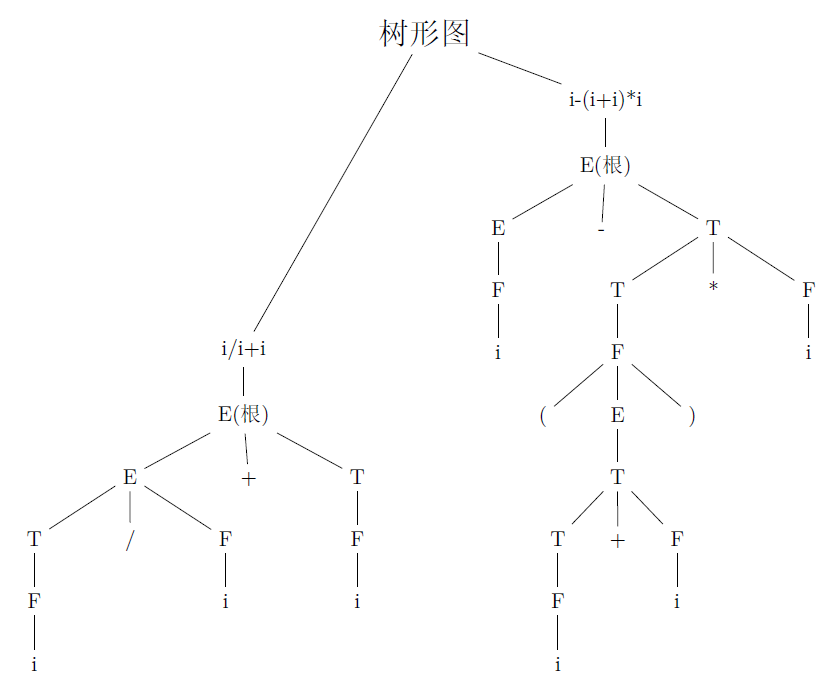
\includegraphics[width=12.5cm,height=9cm]{1.png}
      \caption{树形图表示}
\end{figure}
% \begin{center}
%       \begin{forest}
%             [树形图,s sep = 100,font=\Large[i/i+i,l*=5,for tree = {s sep=(10-level)*2mm}[E(根)[E[T[F[i]]][/][F[i]]][+][T[F[i]]]]]
%                   [i-(i+i)*i,for tree = {s sep=(10-level)*2mm}[E(根)[E[F[i]]][-][T[T[F[(][E[T[T[F[i]]][+][F[i]]]][)]]][*][F[i]]]]]]
%       \end{forest}
% \end{center}
\subsection{}%5
\noindent
证明下面的文法是二义的:$G_5[S]: S \rightarrow iSeS | iS | i$ \\
\begin{align*}
       & S \rightarrow iSeS \rightarrow iiSeS \rightarrow iiSeis \rightarrow iiieii \\
       & S \rightarrow iS \rightarrow iiSeS \rightarrow iiSeiS \rightarrow iiieii   \\
\end{align*}
\begin{center}
      \begin{forest}
            [树形图,s sep = 100,font=\large[iiieii[E(根)[iSeS[i][S[iS[i][i]]][e][S[iS[i][i]]]]]]
                  [iiieii[E(根)[iS[i][iSeS[i][S[i]][e][S[iS[i][i]]]]]]]]
      \end{forest}
\end{center}
\subsection{}%6
\noindent
给出下述文法 $G_7$ , 推导出字符串 $a^nb^nc^n,n>=1 G_7[S]:$
\begin{align*}
       & [1] S \rightarrow aSBA \quad [2] S \rightarrow abB \quad [3] BA \rightarrow AB      \\
       & [4] bA \rightarrow bb  \qquad \ [5] bB \rightarrow bc \quad \ [6] cB \rightarrow cc
\end{align*}
推导过程:
\begin{align*}
      S & \rightarrow aSBA \rightarrow aSAB \rightarrow aabBAB \rightarrow aabABB                 \\
        & \rightarrow aabbBB \rightarrow aabbcB \rightarrow aabbcc \Rightarrow a^2b^2c^2          \\
      S & \rightarrow aSBA \rightarrow aaSBABA \rightarrow aaaSBABABA \rightarrow \cdots          \\
        & \rightarrow a\cdots SBA\cdots \rightarrow a\cdots b\cdots c\cdots \Rightarrow a^nb^nc^n
\end{align*}
\clearpage
\end{document}